\chapter{Secret Key Cryptography}

\section{Introduzione}
La crittografia a chiave segreta richiede l’uso di UNA sola chiave: dato un messaggio (il testo in chiaro) e la chiave, la cifratura produce
dati non intellegibili (il testo cifrato). Il testo cifrato ha circa la stessa lunghezza di quello in chiaro e la decifratura è l’inverso della cifratura, ed usa la stessa chiave. La crittografia a chiave segreta è talvolta chiamata crittografia \textbf{convenzionale} o crittografia \textbf{simmetrica}.
\begin{figure}[htbp]
	\centering%
	\subfigure%
	{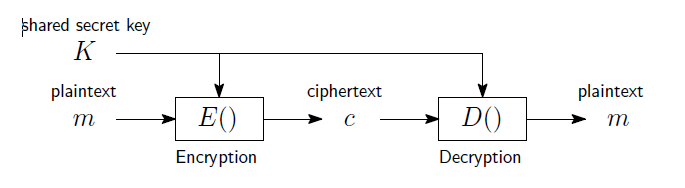
\includegraphics[height=13cm, width=13cm, keepaspectratio]{Immagini/Capitolo2/segreta_schema_blocchi.png}}
	\caption{Schema a blocchi crittografia a chiave segreta \label{fig:segreta_schema_blocchi}} 	
\end{figure}

\subsection{Impieghi crittografia a chiave segreta}
La crittografia a chiave segreta è alla base di molti meccanismi di sicurezza, i suoi principali impieghi sono: 
\begin{itemize}
  \item protezione della \textbf{confidenzialità} (l'uso classico di queste tecniche è rappresentato dalle \textbf{comunicazioni su un canale insicuro}, uno degli usi più moderni invece dalla \textbf{memorizzazione sicura su supporto insicuro})
  \item protezione dell'\textbf{integrità}: tramite queste tecniche possono essere eseguiti test per rilevare eventuali modifiche non consentite.
  \item autenticazione: tramite l'implementazione di protocolli per verificare l'identità di persone e/o processi.
\end{itemize}

\subsubsection{Comunicazioni su un canale insicuro}
In molte circostanze, due entità devono comunicare attraverso un canale insicuro correndo il rischio di essere ascoltate da una terza parte. Questo contesto è molto comune: si pensi alle reti LAN, che trasmettono dati in broadcast. La crittografia a chiave segreta permette a due entità che condividono un segreto (la chiave) di comunicare attraverso un canale insicuro, ove non può essere garantita l’assenza di intercettazioni/ascoltatori (eavesdropper), avendo la garanzia che il contenuto della comunicazione rimarrà confidenziale.

\subsubsection{Memorizzazione sicura}
Si supponga di disporre di un supporto di memorizzazione non protetto (ad esempio accessibile a molti utenti). Se si desidera salvare i dati proteggendone la confidenzialità si può definire una chiave segreta, salvare i dati dopo averli crittografati con tale chiave e custodire la chiave segreta in un luogo protetto. Il rischio dell'uso di questa tecnica consiste nella possibilità di smarrimento della chiave. In tal caso i dati sarebbero irrevocabilmente persi.

\subsubsection{Autenticazione forte}
Per \textbf{autenticazione forte (strong authentication)} si intende che si è in grado di provare la conoscenza di un segreto, che contraddistingue l'identità di una data entità, senza rivelarlo. L'autenticazione forte è ottenibile utilizzando la crittografia a chiave segreta, ed è particolarmente utile quando due processi devono comunicare su una rete insicura. A rigore il segreto che contraddistingue l'identità che si desidera autenticare dovrebbe essere noto solo a quest'ultima. Nella crittografia chiave segreta tale requisito non può essere soddisfatto. Il segreto in questione è una chiave crittografica che deve essere nota anche all'entità autenticante.

\subsubsection{Esempio}
Si supponga che Alice e Bob condividano una chiave segreta $K_{AB}$ e che vogliano autenticarsi reciprocamente, cioè ciascuno vuole accertarsi dell'identità dell'altro. \newline \textbf{ipotesi:} $K_{AB}$ è nota solo ad Alice e Bob. Alice deve dimostrare a Bob di conoscere $K_{AB}$ senza rivelarla e viceversa. \newline \textbf{Strategia a sfida e risposta:} ciascuno dimostra di conoscere $K_{AB}$ rispondendo ad una sfida posta dall'altro. La \textbf{sfida} è un numero/stringa random \textbf{r} non prevedibile e sempre diversa. La \textbf{risposta} alla sfida è la sfida stessa cifrata \textbf{$E(K_{AB},R)$}. In \figurename ~\ref{fig:strong_auth_sec} è riportato un possibile schema di autenticazione a sfida e risposta (challenge-response) a chiave segreta. La procedura segue i seguenti passi:
\begin{itemize}
  \item Alice genera un numero random $r_{A}$ (la sfida) e la invia al presunto Bob
  \item il presunto Bob critta la sfida con la sua chiave segreta $K'_{AB}$ e restituisce ad Alice la risposta $E(K'_{AB}, r_{A})$
  \item Alice riceve la risposta del presunto Bob e la decritta con la chiave $K_{AB}$, cioè calcola $D(K_{AB},E(K'_{AB}, r_{A}))$. Se ottiene $r_{A}$, allora il presunto Bob è realmente Bob poiché con elevatissima probabilità, se $D(K_{AB},E(K'_{AB}, r_{A})) = r_{A}$, allora $K'_{AB} = K_{AB}$. In caso negativo deduce invece che il presunto Bob è un impostore. In modo analogo Bob verifica l'identità di Alice.
\end{itemize}
\begin{figure}[htbp]
	\centering%
	\subfigure%
	{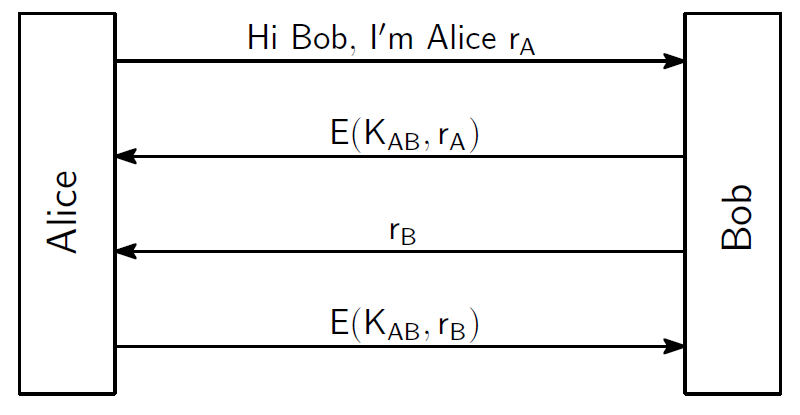
\includegraphics[height=13cm, width=13cm, keepaspectratio]{Immagini/Capitolo2/strong_auth_secret.png}}
	\caption{Schema a blocchi crittografia a chiave segreta \label{fig:strong_auth_sec}} 	
\end{figure}
La sicurezza del precedente protocollo si fonda sulle seguenti condizioni che non devono venire meno:
\begin{itemize}
  \item solo e soltanto Alice e Bob devono conoscere la chiave segreta $K_{AB}$
  \item le sfide generate devono essere \textbf{randomiche}, e di conseguenza non prevedibili, e \textbf{non ripetibili}, cioè la probabilità che due sfide si ripetano deve tendere a zero. L'attaccante potrebbe infatti collezionare molte coppie testo in chiaro/testo cifrato.
  \item è importante quindi che il numero di bit di una sfida sia superiore ad una data soglia (almeno 64 bit)
\end{itemize}

\subsubsection{Controllo di integrità}
La verifica dell’integrità di un messaggio inviato o di un file è un problema ricorrente in telecomunicazioni e in informatica. Per rilevare eventuali modifiche accidentali si fa uso generalmente di codici (somme) di controllo, detti anche \textbf{checksum}. Un \textbf{checksum} associa ad un qualsiasi messaggio $\textbf{m} \in \{0,1\}^*$ un codice di lunghezza prefissato di $b$ bit (generalmente $b = 32,64,128$ bit): $ck(\textbf{m}) \in \{0,1\}^b$. Un buon \textbf{checksum} dovrebbe variare in modo significativo anche a fronte di iminime variazioni dell'input. \newline \newline 
La sorgente del messaggio $m_{s}$ rende pubblico/invia il corrispondente checksum $ck(m_{s})$. Chi riceve il messaggio $m_{r}$ calcola il checksum e verifica se vale l'uguaglianza $ck(m_{s}) = ck(m_{r})$. In caso affermativo, conclude che $m_{s} = m_{r}$. Si noti tuttavia che, seppur improbabile, è possibile ottenere dei falsi positivi, cioè $ck(m_{s}) = ck(m_{r} )$ anche se non è vero.

\subsubsection{Checksum segreti e non segreti}
I codici di controllo servono per proteggere l’hardware da difetti e da inevitabili errori/guasti. Esistono codici di controllo molto sofisticati come i \textbf{CRC (Cyclic Redundancy Check)} per i quali la probabilità di falsi positivi è estremamente ridotta. Esistono anche i codici \textbf{FEC (Forward Error Correction)} che permettono di correggere eventuali errori oltre che a rilevarli (aggiungendo ulteriore ridondanza). Tuttavia entrambe queste tecniche \textbf{non} sono utilizzabili per la protezione contro attacchi intelligenti. Essendo pubblici, infatti, un avversario intelligente che vuole cambiare un messagio potrebbe modificare anche il codice di controllo in maniera coerente.\newline \newline
Per la protezione contro modifiche maliziose ad un messaggio, è richiesto un codice di controllo (checksum) segreto. Se l'algoritmo non è noto, nessuno può calcolare il checksum corretto per il messaggio modificato. Chiaramente, come nel caso degli algoritmi di cifratura, anziché un
algoritmo segreto conviene avere un algoritmo noto a tutti che richiede la conoscenza di una chiave segreta per il calcolo di un codice di controllo (Vedi pagina ~\pageref{sec:openStruct}, principio \textbf{Open Structure}). \newline \newline
In ciò consiste appunto un checksum cifrato, detto anche \textbf{MIC (Message Integrity Code)}. Il funzionamento del MIC è il seguente:
\begin{itemize}
  \item l'algoritmo produce un codice di autenticazione di lunghezza fissa $MIC(K,m)$, denominato anche \textbf{MAC (Message Authentication Code)}
  \item il codice MIC MIC(K,m) viene trasmesso insieme al messaggio m stesso
  \item formalmente l’input è una coppia $(K,m) \in \{0, 1\}^k \times \{0, 1\}^*$, dove $k$ denota il numero di bit della chiave segreta K, mentre l'output è sempre una stringa binaria di lunghezza prefissata, cioè $MIC(K,m) \in \{0, 1\}^b$
\end{itemize}

\subsection{Cifrari a blocchi e cifrari a flusso}
Un \textbf{cifrario a blocchi} elabora un blocco di elementi in ingresso per volta, producendo un blocco di uscita per ciascun blocco di ingresso. Questa metodologia implica quindi che:
\begin{itemize}
  \item il testo in chiaro deve essere preliminarmente suddiviso in blocchi
  \item il testo cifrato si ottiene combinando i vari blocchi cifrati
\end{itemize}
DES, IDEA e AES sono esempi di cifrari a blocchi simmetrici. Un \textbf{cifrario a flusso}, invece, elabora continuamente gli elementi in ingresso, producendo in uscita un "flusso" di elementi cifrati. Gli elementi cifrati vengono prodotti singolarmente, uno alla volta, man mano che la cifratura procede.

\section{Cifratura a blocchi}

\subsection{Introduzione e concetti generali}
L’algoritmo di cifratura converte un blocco di testo in chiaro in un blocco di testo cifrato. La chiave K non deve essere troppo corta (e.g. se K ha lunghezza 4 bit, sono sufficienti $2^4 = 16$ tentativi per individuarla). Analogamente la lunghezza (fissata) di un blocco non deve essere troppo piccola (e.g. se un blocco ha lunghezza 8 bit, ottenendo delle coppie plaintext - ciphertext si potrebbe costruire una tabella di $2^8 = 256$ coppie utilizzabile per la decfiratura).\newline 
D'altra parte, avere blocchi esageratamente lunghi oltre a non essere necessario dal punto di vista della sicurezza, comporta una gestione più complicata e può degradare le prestazioni. \textbf{64 bit è una lunghezza ragionevole per un blocco}: 
\begin{itemize}
  \item è improbabile ottenere ordine di $2^{64}$ coppie $\langle plaintext, ciphertext \rangle$ per costruire una tabella di decifratura, e
  \item anche se fosse possibile, la sua memorizzazione richiederebbe una spazio enorme ($2^{64}$ record da 64 bit),
  \item come pure l’ordinamento per consentire ricerche efficienti
\end{itemize}
Il modo più generale per cifrare un blocco da 64 bit è definire una \textbf{biiezione} $\gamma :\{0,1\}^{64} \rightarrow \{0,1\}^{64}$. Tuttavia, memorizzare la definizione della \emph{biiezione} in una struttura dati è impraticabile: sarebbero richiesti $2^84 \times 64 = 2^{70}$ bit. Ad essere precisi ce ne vogliono un po' di meno, trattandosi di un \textbf{biiezione}, comunque almeno $2^{69}$ bit sono richiesti \textcolor{red}{(perché?!?!)}. Inoltre, così facendo la chiave è incorporata nella biiezione: per renderla parametrica rispetto alla chiave è necessario memorizzare una biiezione per ogni possibile chiave.\newline \newline
I sistemi di crittografia a chiave segreta sono concepiti per usare una chiave ragionevolmente lunga (ad esempio 64 bit e generare una \textbf{biiezione} che appare, a chi non conosce la chiave, completamente \underline{random}. Se la biiezione fosse realmente random due input $i$ e $i'$ nei quali cambia un solo bit (uno qualunque) sarebbero \textbf{statisticamente indipendenti}: non può succedere, ad esempio, che il terzo bit dell'output cambia \textbf{sempre} quando il dodicesimo bit dell'input cambia. Gli algoritmi crittografici sono pensati per \textbf{diffondere/spargere} in tutti i bit dell'output il valore di ogni bit dell'input: si cerca di far si che ogni bit dell'output dipenda allo stesso modo da tutti i bit dell'input.

\subsection{Sostituzione e Permutazione}
Sostituzioni e permutazioni sono due trasformazioni base applicabili ad un blocco di dati.\newline \newline
Si assuma di dover cifrare un blocco di $k$ bit. Una \textbf{sostituzione} specifica, per ciascuno dei $2^k$ possibili valori dell'input, i $k$ bit dell'output. Per specificare una sostituzione \textbf{"completamente random"} sono necessari circa $k2^k$ bit. E' quindi impraticabile implementare una sostituzione per blocchi di $64$ bit, mentre è fattibile per blocchi di lunghezza di $8$ bit. Esempio di crittografia per sostituzione è il \textbf{Cifrario di Cesare}.\newline \newline
Una \textbf{permutazione} specifica, per ciascuna delle $k$ posizioni dei bit in input, la posizione del corrispondente bit nell'output. Per specificare una permutazione \textbf{"completamente random"} per un blocco di
lunghezza $k$ bit sono necessari $k\log_2 k$ bit. Infatti per ciascuno dei k bit va specificata la sua posizione nell'output; ogni posizione richiede $k\log_2 k$. Ad esempio: essendo $2^6 = 64$, sono necessari $6 = \log_2 {64}$ bit per specificare la nuova posizione che l'i-esimo bit in input avrà in output. \newline \newline
Si noti che una \textbf{permutazione} è un caso particolare di \textbf{sostituzione} in cui ogni bit dell'output ottiene il suo valore da esattamente un bit dell'input.

\subsection{Cifrario a blocchi – schema generale}
Un algoritmo di cifratura a chiave segreta può funzionare come segue:
\begin{itemize}
  \item scompone il blocco in input in pezzi più piccoli (e.g. blocchi da 8 bit)
  \item applica una sostituzione (tramite una \textbf{rete combinatoria}) a ciascun pezzo da 8 bit (la sostituzione dipenderà dal valore della chiave)
  \item gli output delle sostituzioni vengono riuniti in un unico blocco (64 bit)
  \item tale blocco viene permutato in un permutatore a 64 bit (che ha il compito di diffondere le modifiche eseguite nelle sostituzioni)
  \item il processo viene ripetuto un certo numero di volte riportando l'output in ingresso
\end{itemize}
%%La scomposizione in blocchi e la ricomposizione vanno effettuate in maniera saggia, al fine di ottimizzare %%efficacia e efficienza del \textbf{cifrario}.
\subsection{Cifrario a blocchi – esempio}
Ogni attraversamento del cifrario viene detto \textbf{round}. In riferimento alla \figurename ~\ref{fig:block_chipher} si fanno le seguenti considerazioni. Con un solo round, un bit $b_x$ di input può influenzare soltanto 8 bit $b_{x1}, b_{x2}, …, b_{x8}$ dell'output, poiché $b_x$ ha attraversato soltanto un blocco di sostituzione. In generale i bit $b_{x1}, b_{x2}, …, b_{x8}$ non sono consecutivi essendo stati mescolati nel permutatore. Alla fine del secondo round, assumendo che i bit $b_{x1}, b_{x2}, …, b_{x8}$ siano smistati in blocchi di sostituzione distinti, il bit $b_x$ iniziale influenza tutti i bit in output.
\begin{figure}[htbp]
	\centering%
	\subfigure%
	{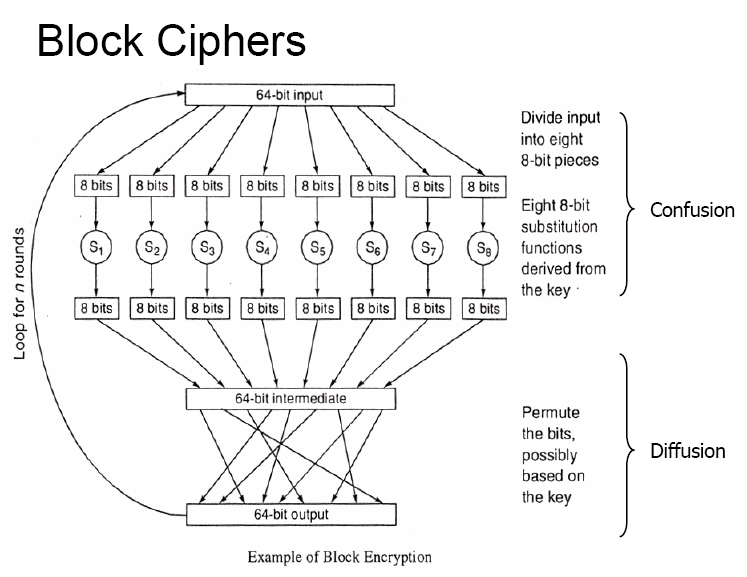
\includegraphics[height=13cm, width=13cm, keepaspectratio]{Immagini/Capitolo2/block_cipher.png}}
	\caption{Schema a blocchi crittografia a chiave segreta \label{fig:block_chipher}} 	
\end{figure}

\section{Data Encryption Standard - DES}
DES fu pubblicato nel 1977 dal \textbf{National Bureau of Standards}, ora rinominato \textbf{N}ational \textbf{I}nstitute of \textbf{S}tandards and \textbf{T}echnology (\textbf{NIST}), per usi commerciali e "altre" applicazioni del governo statunitense. Progettato da IBM, si basa sul precedente cifrario \textit{Lucifer} ed è frutto della collaborazione con consulenti della NSA. DES usa una chiave di 56 bit, e mappa un blocco di input da 64 bit in un blocco di output da 64 bit (l'algoritmo è quindi abbastanza rigido, al contrario di altri cifrari a blocchi). La \textbf{chiave} è in realtà costituita da una sequenza di 64 bit, ma un bit in ogni ottetto (il blocco da 64 bit è formato da 8 sequenze di 8 bit dette ottetti) è usato come \textbf{odd parity} su ciascun ottetto. Di fatto, soltanto 7 bit in ogni ottetto sono quindi veramente significativi come chiave. \newline \newline

DES è efficiente se realizzato in hardware, ma relativamente lento se implementato in software. Sebbene l'essere difficilmente implementabile come software non fosse un requisito specificato nel progetto molti sostengono che in realtà questa mancanza fosse voluta, forse per limitarne l'uso ad organizzazioni in grado di realizzare sistemi hardware, o forse perché rese più facile controllare l'accesso alla tecnologia. Ad ogni modo, l'aumento delle capacità di calcolo delle CPU rese possibile realizzare una versione software di DES. Una 500-MIPS (Million Instruction Per Second) CPU può infatti cifrare ad un tasso di circa 30 KB/s e forse più, a seconda dei dettagli architetturali della CPU e dell'intelligenza dell'implementazione. Un processore Intel Core i7 Extreme Edition i980EE ha una capacità di calcolo di circa 150 MIPS, quindi può cifrare ad un tasso di circa 9 KB/s (per cifrare 1 MB impiega circa 110 secondi). L’implementazione software è pertanto attualmente adeguata a molte applicazioni.\newline \newline

\subsection{Perché chiavi da 56 bit?}
La scelta di una chiave da 56 bit causò molte controversie. Prima che DES fu adottato, le persone al di fuori della \textit{intelligence community} lamentavano che 56 bit non offrivano una sicurezza adeguata. Perché solo 56 dei 64 bit di una chiave DES sono effettivamente usati nell'algoritmo? Lo svantaggio di usare 8 bit della chiave per un controllo di parità è che ciò rende DES molto meno sicuro (256 volte meno sicuro contro una ricerca esaustiva). Ma qual è il vantaggio di usare 8 bit per un controllo di parità? Una possibile risposta è che permette di verificare che la chiave non sia corrotta. Tuttavia questa spiegazione non regge. Se si considerassero infatti 64 bit a caso invece della chiave, c'è una probabilità su 256 che il controllo di parità dia esito positivo. La probabilità che la chiave sia comunque errata (nonostante il controllo di parità dia esito positivo) è troppo alta. Inoltre avere una chiave corrotta non comporta un problema di sicurezza, semplicemente la cifratura/decifratura non viene eseguita correttamente. Chiaramente è anche ridicolo sostenere che la scelta di 56 bit sia stata fatta per risparmiare memoria. \newline La risposta ormai condivisa è che il governo statunitense abbia deliberatamente indebolito la sicurezza di DES di una quantità appena sufficiente da consentire alla NSA di violarlo.

\subsection{Violabilità e sicurezza di DES}
Gli avanzamenti tecnologici dell'industria dei semiconduttori hanno reso ancora più critico il problema della lunghezza della chiave di DES. la velocità dei chip e un po' di furbizia permettono di violare (individuare) le chiavi DES con approcci a forza bruta in tempi ragionevoli. Il rapporto prestazioni/prezzo dell'hardware cresce del
$40\%$ per anno. La lunghezza delle chiavi dovrebbe aumentare di 1 bit ogni 2 anni. Assumendo che 56 bit erano appena sufficienti nel 1979 (quando DES fu standardizzato), 64 bit erano adeguati nel 1995, e 128 bit dovrebbero essere sufficienti fino al 2123. \newline \newline Ragioniamo ora sulla sicurezza di DES. Se si dispone di un singolo blocco $\langle plaintext,ciphertext \rangle$ quanto è difficile trovare la chiave? Un approccio a forza bruta dovrebbe provare ordine di $2^{56} \approx 10^{17}$ chiavi. Se ogni tentativo richiede una singola istruzione sono necessarie ordine di 1000 MIPS-year istruzioni.
\begin{itemize}
  \item 1 MIPS = 1 Milionef di Istruzioni Per Secondo
  \item 1 MIPS-year = numero di istruzioni eseguite in un anno ad un tasso pari a 1 MIPS
  \item 1 MIPS-year = 1 MIPS $\times(365 \times 86400)$ secondi in un anno = $3,1536 \times 10^{13}$ istruzioni
  \item $2^{56} \approx 10^{17} \approx 10^{3}$ MIPS-year
\end{itemize}
Questo vale tuttavia \textbf{SOLO} per effettuare una ricerca esaustiva. Dopo di che entra in gioco il fatto che io sappia riconoscere o meno il testo in chiaro.
\subsection{Violabilità DES - esempio}
Anche nell'ipotesi più scomoda per l'avversario di disporre solo di testo cifrato (in ragionevole quantità), un attacco a forza bruta è ancora possibile. Se ad esempio l'avversario sa soltanto che il testo in chiaro è ASCII a 7 bit ogni volta che prova una chiave deve verificare se sono nulli tutti i bit nelle posizioni $8, 16, 24, ..., n \times 8, ...$. Per ogni blocco di 64 bit, vanno esaminati solo 8 bit; i bit in posizione 8, 16, 24, 32, 40, 48, 56, 64. Se almeno uno di questi bit vale 1 la chiave è sicuramente errata. in caso contrario nulla si può dire; \textbf{la probabilità di errore è pertanto 1 su 256 ossia la probabilità che tutti questi bit valgano 0}. Se l'avversario esamina diversi blocchi, ad esempio 10, e verifica che si tratta sempre di ASCII a 7 bit la probabilità che la chiave scelta sia errata si riduce a 1 su 2560. Si noti che gli attuali chip commerciali che implementano DES non si prestano a ricerche esaustive della chiave: sono pensati per cifrare molti dati con una stessa chiave. Infatti il caricamento di una chiave è un'operazione lenta se confrontata con la velocità con la quale viene eseguita la cifratura dei dati. Tuttavia è sempre possibile costruire un chip ottimizzato ad eseguire ricerche esaustive della chiave.

\subsection{Violabilità DES - cifratura multipla}
Per ovviare a tali problemi di sicurezza è possibile cifrare più volte e con diverse chiavi lo stesso blocco di dati. Si parla di \textbf{cifratura multipla (multiple encryption)}. Si ritiene che una cifratura con un triplo DES sia
$2^{56}$ volte più difficile da violare.

\subsection{DES - Struttura base}
\begin{figure}[htbp]
	\centering%
	\subfigure%
	{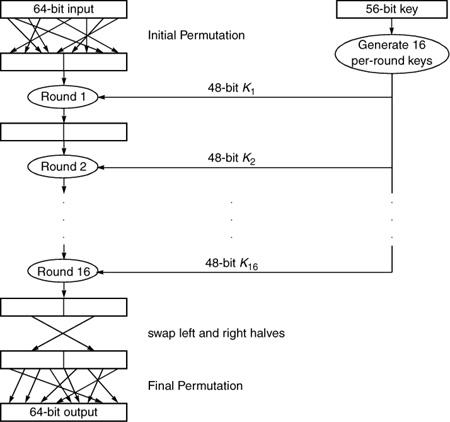
\includegraphics[height=10cm, width=13cm, keepaspectratio]{Immagini/Capitolo2/des_structure.png}}
	\caption{Schema a blocchi DES \label{fig:des_struct}} 	
\end{figure}
La struttura di base dell'algoritmo DES è descritta in \figurename ~\ref{fig:des_struct}. In estrema sintesi:
\begin{itemize}
  \item L'input di 64 bit è sottoposto ad una permutazione iniziale;
  \item La chiave da 56 bit viene usata per generare 16 per-round chiavi da 48 bit; una chiave per ciascuno dei 16 round, prendendo 48 differenti sottoinsiemi dei 56 bit della chiave
  \item Ogni round riceve in input l'output di 64 bit del round precedente e la chiave da 48 bit di quel round
  \item Ogni round restituisce un output di 64 bit
  \item Dopo il 16-esimo round, le due metà dell'output di 64 bit vengono scambiate e il risultato viene sottoposto ad un’altra permutazione (inversa a quella iniziale)
  \item La decifratura consiste semplicemente nell’eseguire la cifratura DES all’indietro
  \item Per decifrare un blocco è necessario applicare la permutazione iniziale (ciò annulla l’effetto della permutazione finale), generare le 16 chiavi di round, che andranno usate in ordine inverso (prima $K_{16}$, l'ultima chiave generata), seguire 16 round esattamente come nella cifratura, scambiare le due metà dell'output e sottoporle a un'altra permutazione (che annulla l'effetto della permutazione iniziale)
\end{itemize}
Per descrivere DES è quindi sufficiente discutere le permutazioni iniziale e finale, come le chiavi di round sono generate, e cosa succede durante un round.


\subsection{DES - Permutazioni dei dati}
L'operazione di permutazione è molto importante in quanto diffonde la dipendenza dei bit in/out. Nel caso di DES però le permutazioni finale e iniziale non hanno effetto. Dimostriamo tale affermazione. \newline
\begin{figure}[htbp]
	\centering%
	\subfigure%
	{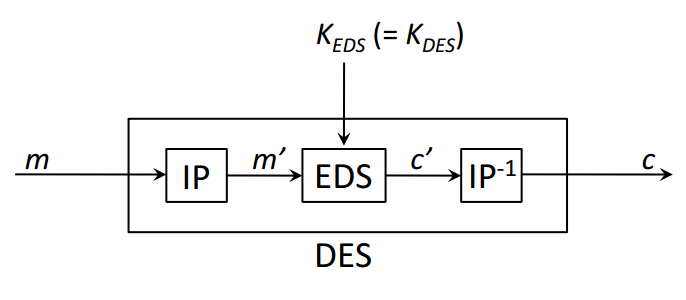
\includegraphics[height=10cm, width=8cm, keepaspectratio]{Immagini/Capitolo2/des_perm_3.png}}
	\caption{Inutilità delle permutazioni iniziale e finale \label{fig:des_perm_3}} 	
\end{figure}
Supponiamo di non averle. Se assumiamo per assurdo che il cifrario cosi ottenuto sia facile da violare, vogliamo dimostrare che anche DES è facile da violare. Chiamiamo il cifrario senza permutazione EDS. Se posso violare EDS (disponendo, ad esempio, di una coppia $\langle plaintext, ciphertext \rangle$), basta permutare ciò che ottengo e violo DES. Infatti, sia $\langle m, c \rangle$ una coppia $\langle plaintext, ciphertext \rangle$ di DES. Si consideri allora la coppia $\langle m', c' \rangle$, dove m' e c' sono ottenuti applicando la permutazione iniziale ad m e c. Allora, la chiave $K_{EDS}$ che si ottiene violando EDS per la
coppia $\langle m', c' \rangle$ coincide con la chiave $K_{DES}$ di DES per la
coppia $\langle m, c \rangle$ (vedi \figurename ~\ref{fig:des_perm_3}). L'ipotesi è che tali permutazioni siano state introdotte per rendere più complicata una possibile implementazione software.
\begin{figure}[htbp]
	\centering%
	\subfigure%
	{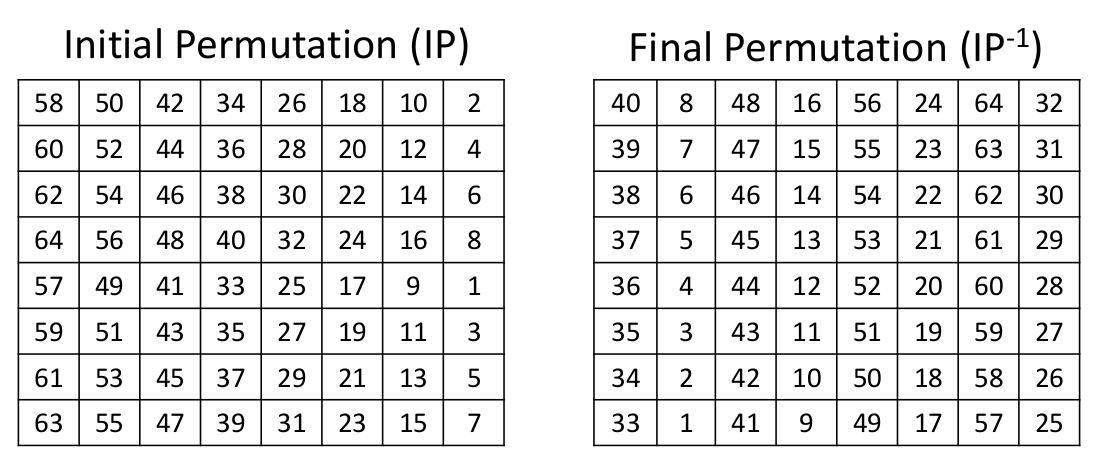
\includegraphics[height=10cm, width=13cm, keepaspectratio]{Immagini/Capitolo2/des_perm.png}}
	\caption{Tabella permutazioni DES \label{fig:des_perm}} 	
\end{figure}
Come sono state definite quindi le permutazioni iniziale e finale? E' di fatto una permutazione regolare, come è mostrato in \figurename ~\ref{fig:des_perm}. Le tabelle vanno interpretate nel seguente modo: i numeri, da 1 a 64, riportati in tabella rappresentano le posizioni dei bit in input alla permutazione, mentre l’ordine (per righe da sx verso dx) dei numeri nella tabella rappresenta la corrispondente posizione dei bit in output. Ad esempio, la permutazione iniziale sposta il 58-esimo bit in input nel primo bit in output, e il 50-esimo bit in input nel secondo bit in output. Non si tratta di permutazioni generate in modo random, in quanto presenta delle evidenti regolarità, come è evidenziato in \figurename ~\ref{fig:des_perm_2}.
\begin{figure}[htbp]
	\centering%
	\subfigure%
	{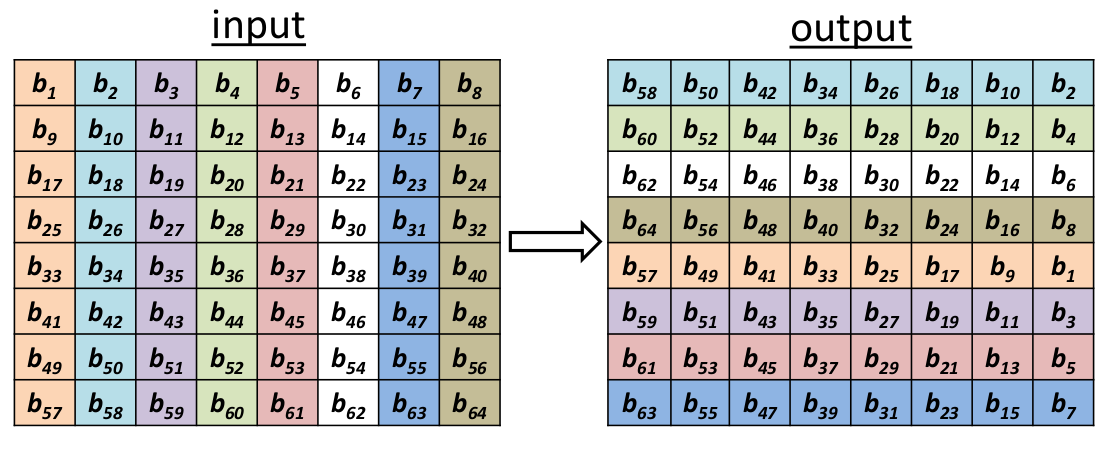
\includegraphics[height=10cm, width=10cm, keepaspectratio]{Immagini/Capitolo2/des_perm_2.png}}
	\caption{Regolarità tabella permutazioni DES \label{fig:des_perm_2}} 	
\end{figure}
\subsection{DES - Generazione chiavi di round}
DES genera sedici chiavi di round da 48 bit a partire dalla chiave principale K di 64 bit nominali, di cui solo 56 effettivi. I bit di parità di K non vengono infatti considerati. Denoteremo con $K_{1}$,$K_{2}$,...,$K_{16}$ le sedici chiavi di round. Il procedimento è il seguente:
\begin{itemize}
  \item viene prima effettuata una permutazione iniziale sui 56 bit effettivi di K
  \item i 56 bit in output vengono divisi in due metà $C_{0}$ e $D_{0}$
  \item Le sedici chiavi vengono generate in sedici round, i.e. nell'i-esimo round viene generata la chiave di round $K_{i}$
\end{itemize}
\subsubsection{Permutazione iniziale}
\begin{figure}[htbp]
	\centering%
	\subfigure%
	{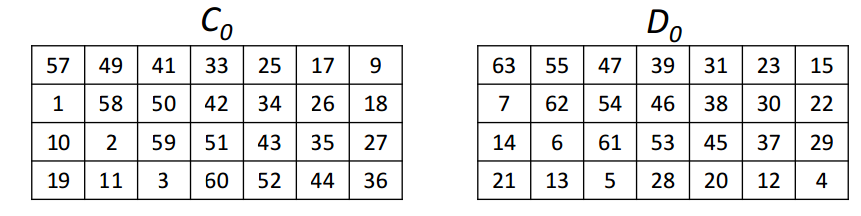
\includegraphics[height=10cm, width=10cm, keepaspectratio]{Immagini/Capitolo2/des_perm_keys.png}}
	\caption{Permutazione iniziale della chiave \label{fig:des_perm_keys}} 	
\end{figure}
\begin{figure}[htbp]
	\centering%
	\subfigure%
	{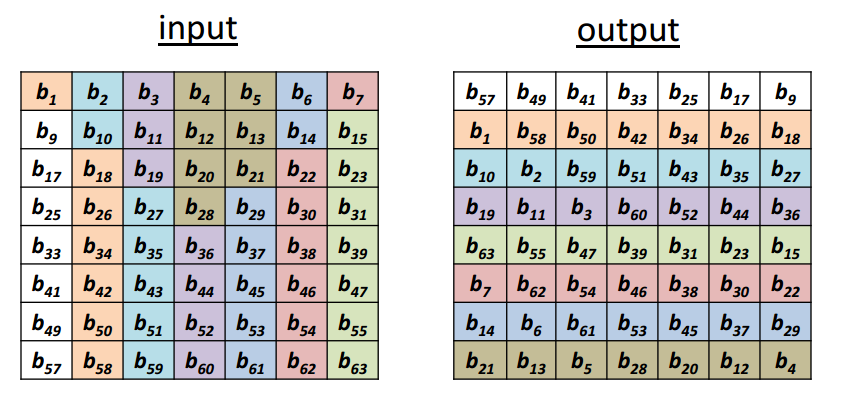
\includegraphics[height=10cm, width=10cm, keepaspectratio]{Immagini/Capitolo2/des_perm_keys_2.png}}
	\caption{Regolarità tabella permutazioni delle chiavi DES \label{fig:des_perm_keys_2}} 	
\end{figure}
La struttura della permutazione iniziale della chiave è illustrata in \figurename ~\ref{fig:des_perm}. Il valore numerico di un elemento della tabella rappresenta la posizione del bit in input, mentre l’ordine nella tabella rappresenta la posizione del bit in output (come per le permutazioni dei dati). Anche in questo caso non è random, in quanto presenta delle evidenti regolarità, come è evidenziato in \figurename ~\ref{fig:des_perm_keys_2}. Come nel caso delle permutazioni iniziale e finale dei dati, non apportano alcun miglioramento alla sicurezza.
\newpage
\subsubsection{Generazione $K_{i}$ nell'i-esimo round}
\begin{figure}[htbp]
	\centering%
	\subfigure%
	{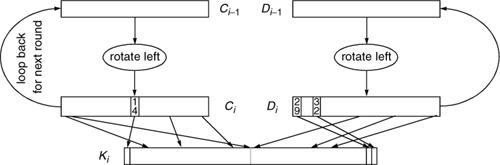
\includegraphics[height=10cm, width=10cm, keepaspectratio]{Immagini/Capitolo2/round_i.png}}
	\caption{generazione di Ki: round i \label{fig:round_i}} 	
\end{figure}
Trattiamo ora la generazione della chiave $K_{i}$ che avviene nell'i-esimo round. La procedura avviene seguendo questi passi (come mostrato in \figurename ~\ref{fig:round_i}):
\begin{itemize}
  \item i bit delle due metà $C_{i-1}$ e $D_{i-1}$ della (i-1)-esima chiave $K_{i-1}$ vengono ruotati (traslazione ciclica) a sinistra. L'entità della traslazione a dipende dal round: nei round 1, 2, 9 e 16 si ha una rotazione a sinistra di un solo bit (i.e. il primo bit diventa l’ultimo bit a destra), mentre negli altri round si ha una rotazione a sinistra di due bit.
  \item la permutazione di $C_{i}$ che produce la metà sinistra di $K_{i}$ è illustrata sotto. Si noti che i bit in posizione 9, 18, 22, e 25 sono scartati.
  	\begin{table}[h]
  	\centering
	\begin{tabular}{llllll}
	14 & 17 & 11 & 24 & 1  & 5  \\
	3  & 28 & 15 & 6  & 21 & 10 \\
	23 & 19 & 12 & 4  & 26 & 8  \\
	16 & 7  & 27 & 20 & 13 & 2 
	\end{tabular}
	\end{table}
  \item la permutazione di $D_{i-1}$ ruotato, cioè di $D_{i}$ , che produce la metà destra di $K_{i}$ è illustrata sotto. Si noti che i bit in posizione 35, 38, 43, e 54 sono scartati; rimangono così 24 bit anziché 28.
  	\begin{table}[h]
  	\centering
	\begin{tabular}{llllll}
	41 & 52 & 31 & 37 & 47 & 55  \\
	30 & 40 & 51 & 45 & 33 & 48 \\
	44 & 49 & 39 & 56 & 34 & 53  \\
	46 & 42 & 50 & 36 & 29 & 32 
	\end{tabular}
	\end{table}
\end{itemize}
\subsection{Un round di DES}
\begin{figure}[htbp]
	\centering%
	\subfigure%
	{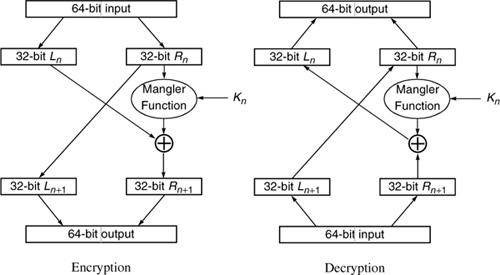
\includegraphics[height=10cm, width=9cm, keepaspectratio]{Immagini/Capitolo2/round_des.png}}
	\caption{Struttura di un round di DES \label{fig:round_des}} 	
\end{figure}
La struttura di un round di des è illustrata in \figurename ~\ref{fig:round_des}). I 64 bit in input sono divisi in due metà da 32 bit: $L_{n}$, la metà sinistra dopo l'(n-1)-esimo round, e $R_{n}$, la metà destra dopo l'(n-1)-esimo round. L'output di 64 bit del round si ottiene concatenando le due metà: $L_{n + 1}$, la metà sinistra dopo l'n-esimo round, e $R_{n + 1}$, la metà destra dopo l'n-esimo round. $L_{n+1}$ è semplicemente $R_{n}$, mentre $R_{n + 1}$ è ottenuto come segue:
\begin{itemize}
  \item $R_{n}$ e $K_{n}$ sono posti in input alla mangler function; la mangler function viene anche detta funzione di Feistel
  \item l'output della mangler function, $mangler(R_{n}, K_{n})$, è una quantità di 32 bit; si noti che $R_{n}, K_{n}$ sono composti da
32 e 48 bit rispettivamente
  \item l'output $mangler(R_{n}, K_{n})$ viene poi sommato (XOR) con $L_{n}$
  \item il risultato ottenuto è $R_{n+1} = mangler(R_{n}, K_{n}) \oplus L_{n}$
\end{itemize}
Si noti che ogni round di DES è facilmente invertibile: noti $L_{n+1}$ , $R_{n+1}$ e $k_{n}$ è facile ottenere $L_{n}$ e $R_{n}$. Infatti $R_{n} = L_{n+1}$ e, poiché $R_{n+1} = mangler(R_{n}, K_{n}) \oplus L_{n}$, risulta $R_{n+1} \oplus mangler(R_{n}, K_{n}) = L_{n}$ (in virtù della proprietà dello XOR secondo cui $x \oplus y \oplus y = x$). La mangler function non è quindi mai utilizzata in senso inverso. DES è elegantemento progettato in modo da essere facilmente invertibile senza richiedere l'invertibilità della mangler function. Esaminando attentamente la \figurename ~\ref{fig:round_des}), si evince che la decifratura è di fatto identica alla cifratura, tranne per il fatto che le due metà da 32 bit sono invertite. In altre parole, fornendo $R_{n+1} \mid L_{n+1}$ in input al round n si ottiene $R_{n} \mid L_{n}$ in uscita
\subsection{Mangler Function}
\begin{figure}[htbp]
	\centering%
	\subfigure%
	{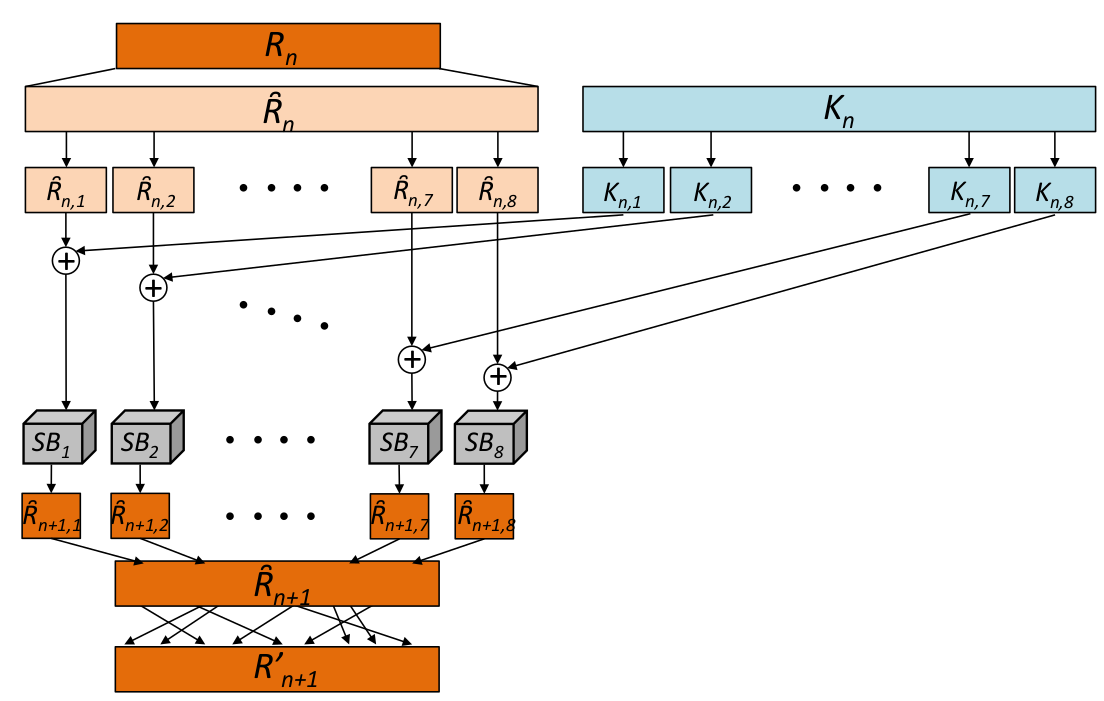
\includegraphics[height=11cm, width=11cm, keepaspectratio]{Immagini/Capitolo2/mangler.png}}
	\caption{Mangler function \label{fig:mangler}} 	
\end{figure}
La mangler function prende in input i 32 bit di $R_{n}$, o R per semplificare, e i 48 bit della chiave $K_{n}$ , o K per semplificare. Produce un output da 32 bit che sommato (XOR) con $L_{n}$ permette di ottenere $R_{n+1}$ (il prossimo R).\newline
La prima operazione è l’espansione di R, da 32 bit a 48 bit. R è scomposto in otto pezzi da 4 bit $R = \lbrace r_{1} , r_{2}, ..., r_{8} \rbrace$. L’i-esimo pezzo $r_{i}$ viene espanso a 6 bit aggiungendo in testa e in coda rispettivamente l’ultimo bit di $r_{i-1}$ e il primo bit di $r_{i+1}$. $r_{1}$ e $r_{8}$ sono considerati adiacenti, cioè $r_{0} = r_{8}$ e $r_{9} = r_{1}$. (Fare riferimento alla \figurename ~\ref{fig:mangler_exp})).
\begin{figure}[htbp]
	\centering%
	\subfigure%
	{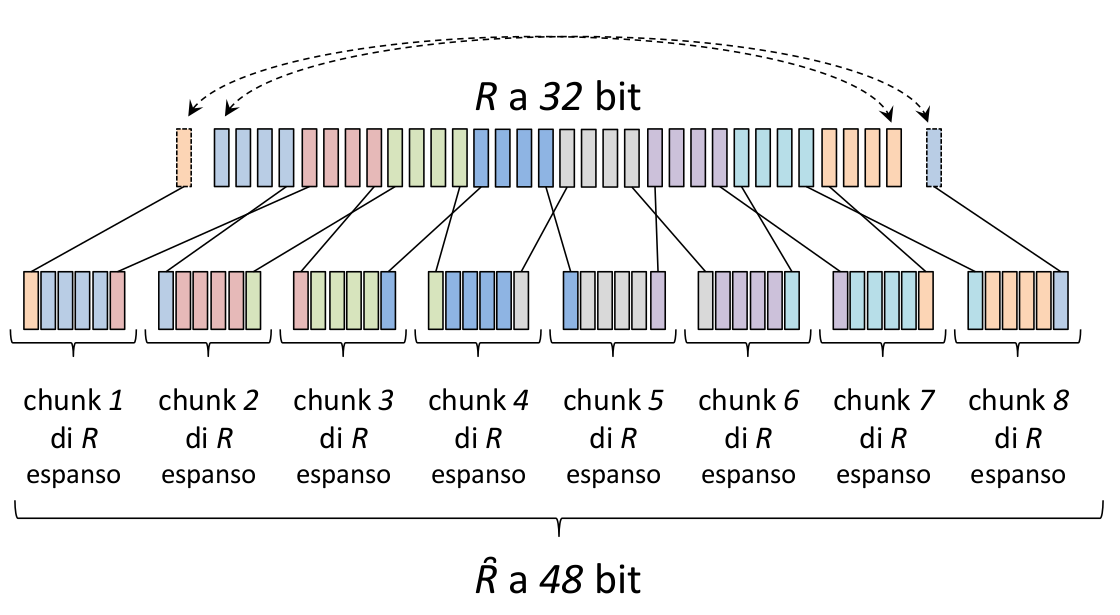
\includegraphics[height=11cm, width=11cm, keepaspectratio]{Immagini/Capitolo2/mangler_exp.png}}
	\caption{Mangler function - espansione \label{fig:mangler_exp}} 	
\end{figure}
\newline
la chiave K($K_{n}$) viene scomposta in otto chunk (pezzi) da 6 bit. L'i-esimo chunk di R($R_{n}$) espanso viene sommato (XOR) all’i-esimo chunk di K. L'output a 6 bit ottenuto viene sottoposto ad una sostituzione \textbf{S-box} che produce un output di 4 bit. Vi sono in tutto otto S-box distinte; l’i-esima S-box elabora la somma dell’i-esimo chunk di K e di R. Ogni S-box ha 64 possibili input e 16 possibili output. Ovviamente input diversi possono essere mappati nello stesso output (sto riducendo lo spazio). Le S-box sono definite in modo tale che esattamente quattro
input distinti sono mappati in ciascun output possibile. Ogni S-box può riguardarsi come quattro S-box separate aventi 4 bit sia in input che in output: i quattro bit in input corrispondono ai bit interni (dal secondo al quinto) dell'input globale, e i due bit esterni (primo e sesto) dell’input globale servono a selezionare quale dei quattro output ottenuti rappresenta l'output globale.
\begin{figure}[htbp]
	\centering%
	\subfigure%
	{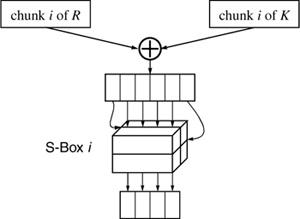
\includegraphics[height=7cm, width=7cm, keepaspectratio]{Immagini/Capitolo2/sbox.png}}
	\caption{S-Box \label{fig:sbox}} 	
\end{figure}
Infine gli otto output, da 4 bit, delle otto S-box sono riuniti in un unico output a 32 bit che viene sottoposto ad una permutazione. Tale permutazione aumenta il livello di sicurezza perché le sostituzioni fatte in ciascuna S-box in un round di DES vengono diffuse negli input di più S-box nel round seguente. Senza tale permutazione, un bit nella parte sinistra dell'input influenzerebbe principalmente alcuni bit della parte sinistra dell'output. Tale permutazione è mostrata in \figurename ~\ref{fig:sbox_perm}).
\begin{figure}[htbp]
	\centering%
	\subfigure%
	{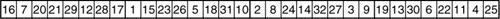
\includegraphics[height=2cm, width=10cm, keepaspectratio]{Immagini/Capitolo2/sbox_perm.png}}
	\caption{Permutazione output S-Box \label{fig:sbox_perm}} 	
\end{figure}